\documentclass[11pt,twoside]{report}
\usepackage[letterpaper,margin=0.8in,top=0.9in]{geometry}  % --- 
%\geometry{textwidth=17cm,margin=2cm}                      % --- 

\usepackage{booktabs}
\usepackage[spanish]{babel}
\usepackage{graphicx}                              % --- 
\usepackage{setspace}                                      % --- 
\usepackage[T1]{fontenc}                                   % --- 
\usepackage[utf8]{inputenc}                                % --- 
\usepackage{blindtext, xfrac}                              % --- 
\usepackage{siunitx}                                      % --- 
\usepackage{parskip}                                       % --- 
\usepackage{lastpage}                                      % --- 
\usepackage{multirow,array,tabularx}                       % --- 
\usepackage{enumitem}                                      % --- 
\usepackage{framed}                                        % ---
\usepackage{lipsum}                                        % ---
\usepackage{listings}                                      % ---
\usepackage{float}

\usepackage[sfdefault,scaled=.85]{FiraSans}
\usepackage{newtxsf}

\bibliographystyle{apalike}

\usepackage[pdfpagelabels,final,bookmarks=true,plainpages=false]{hyperref}
\usepackage[dvipsnames,svgnames,x11names]{xcolor}
\hypersetup{colorlinks=true,citecolor=BlueViolet,linkcolor=Blue,urlcolor=PineGreen,filecolor=Green}
% -------------------------------------------------------------------------
\usepackage[spanish]{cleveref}  % debe ser cargado despues de hyperref
\input{crefnames.tex}
% -------------------------------------------------------------------------
\definecolor{backcolour}{RGB}{242,242,242}   % gris claro de fondo
\definecolor{codegray}{RGB}{128,128,128}     % gris medio para números
\definecolor{codegreen}{RGB}{0,128,0}        % verde para comentarios
\definecolor{codepurple}{RGB}{128,0,128}     % púrpura para strings
\lstdefinestyle{mystyle}{
    backgroundcolor=\color{backcolour},   
    commentstyle=\color{codegreen},
    keywordstyle=\color{magenta},
    numberstyle=\tiny\color{codegray},
    stringstyle=\color{codepurple},
    basicstyle=\ttfamily\footnotesize,
    breakatwhitespace=false,         
    breaklines=true,                 
    captionpos=b,                    
    keepspaces=true,                 
    numbers=left,                    
    numbersep=5pt,                  
    showspaces=false,                
    showstringspaces=false,
    showtabs=false,                  
    tabsize=2
}

\lstset{style=mystyle}

\DeclareSIUnit\lpm{\liter\per\minute}

\DeclareGraphicsExtensions{.pdf,.png,.jpg}

\setcounter{secnumdepth}{3}

\newcommand{\uncol}{Universidad Nacional de Colombia}
\newcommand{\facingbog}{Facultad de Ingeniería - Sede Bogotá}
\newcommand{\dimmbog}{Departamento de Ingeniería Mecánica y Mecatrónica}
\newcommand{\module}{Métodos Numéricos}
\newcommand{\reportType}{Informe Taller 03}
\newcommand{\reportSubject}{Facultad de Ingeniería}


\renewcommand{\thesection}{\arabic{section}}
\renewcommand{\thesubsubsection}{\arabic{section}\arabic{subsection}\arabic{subsubsection}}
\renewcommand*\familydefault{\sfdefault} %% Only if the base font of the document is to be sans serif
\renewcommand{\familydefault}{\sfdefault}
\setlength{\parindent}{0pt} % Default is 15pt.
\setlength{\parskip}{1ex}   % Default is      


\usepackage{fancyhdr}
\usepackage{lastpage}

\pagestyle{fancy}

\fancyhf{} % limpia encabezados y pies
\pagenumbering{arabic}
\fancyfoot[R]{\footnotesize Página \arabic{page} de \pageref{LastPage}}
\fancypagestyle{firststyle}
{
  \fancyhf{}
  \fancyfoot[R]{\footnotesize Página \arabic{page}\ de \pageref{LastPage}}
}

\fancypagestyle{declarationstyle}
{
  \fancyhf{}
  %\fancyfoot[L]{\footnotesize }
  \fancyfoot[C]{\footnotesize \reportType - \module}
  %\fancyfoot[R]{\footnotesize Página \thepage\ de \pageref{LastPage}}
}

\fancyhead{} % clear all header fields
\fancyhead[RO]{\footnotesize \module - \reportType}
\fancyhead[LE]{\footnotesize \reportSubject}
\fancyfoot{} % clear all footer fields
\fancyfoot[L]{\footnotesize Semestre 01 / 2026}

\fancyfoot[R]{\footnotesize Página \thepage\ de \pageref{LastPage}}
\renewcommand{\headrulewidth}{0.4pt}
\renewcommand{\footrulewidth}{0.4pt}

\newenvironment{leftbox}[1]
 {\itemize[
    nosep,
    leftmargin=2pt,
    rightmargin=\dimexpr\textwidth-#1\relax,
    itemindent=\parindent,
    listparindent=\parindent,
  ]\item[]\relax}
 {\enditemize}

\newenvironment{rightbox}[1]
 {\itemize[
    nosep,
    leftmargin=\dimexpr\textwidth-#1\relax,
    rightmargin=2pt,
    itemindent=\parindent,
    listparindent=\parindent,
  ]\item[]\relax}
 {\enditemize}

\definecolor{softBackGround}{RGB}{170,207,238}

\begin{document}

\pagenumbering{Alph}
\begin{titlepage}
\center

\vspace*{-12mm}
{\huge \textbf{\textsc{\uncol}}}\\
{\Large \textbf{\textsc{\facingbog}}}\\[20mm]

\vfill


\includegraphics[width=0.2\textwidth]{./templateFigures/escudo.png}\\[20mm]

\vfill

\begin{framed}
{\Huge \textbf{\reportSubject}}\\[4mm]
{\huge \textbf{\reportType}}\\[4mm]
{\huge \textbf{\module}}
\end{framed}
\vspace{12mm}

\vfill

{\Large \textbf{Coordinacion curso:}}\\[4mm]
{\large Principal: Ing. Daniel Felipe Rodriguez Ramirez\\[14mm]}

{\Large \textbf{Estudiantes/Autores}}\\[4mm]
{\large Nicolás Godoy $<$ngodoya@unal.edu.co$>$ $<$1013113408$>$}\\[2mm]
{\large Sofia Gonzalez $<$lagonzalezvi@unal.edu.co$>$ $<$1011098142$>$}\\[2mm]


\vspace{2.5cm}

11 de mayo de 2026
\end{titlepage}

\newpage
\pagenumbering{arabic}   % <-- IMPORTANTE
\setcounter{page}{1}
\section*{Introducción y Motivación}
El siguiente taller esta realizado en formato \LaTeX para mayor comodidad a la hora de presentar el procedimiento en cada ejercicio para llegar a su respectiva solución. La resolución de los códigos de los ejercicios se realizó en Python y, en los casos en los que se requería, se utilizó Excel; en el presente documento se explican los códigos utilizados; sin embargo, para mayor profundidad en ellos, en los anexos se incluye el cuadernillo de Jupyter \cite{Jupyter} o la respectiva hoja de cálculo, donde se mostraran los códigos con mayor profundidad. Aquí se realiza la explicación y la idea de como se llega a la solución mostrada en el documento.
La regresión logística es uno de los modelos más usados para resolver problemas o situaciones que siguen una distribución de Bernoulli, más conocidos como problemas de clasificación binaria: situaciones en las que, a partir de ciertas variables medibles, se quiere estimar la probabilidad de que ocurra o no un evento (sí/no, pasa/no pasa, 0/1, éxito/fracaso). Estos problemas son bastante comunes en la estadística y su estructura matemática siempre es la misma, independientemente de su dominio: se tienen variables explicativas y una variable de respuesta binaria, y el objetivo es ajustar los parámetros de un modelo probabilístico que explique de la mejor manera posible los datos observados.

Basado en el interés de ambos integrantes en la estadística, en el presente proyecto se aborda esa tarea de ajuste/calibre de los parámetros de un modelo de regresión logística, utilizando un conjunto de datos sintético generado a partir de una relación logística conocida de antemano. Estos datos sintéticos fueron generados con base en una relación conocida (en este caso una ecuación), por lo que es posible verificar con precisión qué tan bien cada método recupera los parámetros buscados. 

El ajuste de los parámetros de este tipo de modelos no tiene una solución algebraica cerrada, es decir, no existe una fórmula que dé directamente los valores óptimos, por lo que se hace necesario recurrir a un método iterativo, como ocurre en la cotidianidad. 

Entre los métodos estudiados en el curso se encuentran el descenso del gradiente y el método de Newton-Raphson, los cuales, a pesar de tener diferencias entre sí, pueden aplicarse al mismo tipo de problema; el primero corresponde a un método de primer orden, en donde cada iteración se mueve en la dirección opuesta al gradiente de la función de costo, usando un tamaño de paso fijo (la tasa de aprendizaje). El segundo, por su parte, es un método de segundo orden que, además del gradiente, usa también la curvatura de la función (la matriz hessiana) para dar un paso un poco más acertado en cada iteración. Por su parte, la librería scikit ofrece distintas herramientas para la optimización de parámetros en problemas de clasificación binaria, por ejemplo, modelos ideales como regresión logística (LogisticRegression).

La comparación de ambos métodos, aplicados exactamente al mismo problema, permite comparar un aspecto esencial en la escogencia de un método para una optimización numérica: el costo computacional de cada iteración frente a la velocidad con la que el método converge o se acerca a la solución
La regresión logística no se limita únicamente al ámbito educativo o al rendimiento académico de estudiantes; su fundamentación matemática como modelo de respuesta binaria la convierte en una herramienta fundamental en múltiples disciplinas. Por ejemplo, en el campo de la salud y la epidemiología, permite estimar la probabilidad de que un paciente desarrolle o presente una determinada enfermedad (p. ej., presencia o ausencia de diabetes, riesgo de infarto) a partir de covariables biomédicas como la presión arterial, la edad o los niveles de glucosa. De manera análoga, en ingeniería de calidad predice la probabilidad de falla en una pieza industrial, y en finanzas evalúa el riesgo de impago de un crédito. Esta transversalidad convierte el estudio numérico de la calibración de sus parámetros en un problema relevante para la práctica profesional.
\section{Planteamiento del problema}

\subsection{Contexto y pregunta de investigación}
El problema abordado consiste en calibrar los parámetros de un modelo de regresión logística a partir de un conjunto de datos observados usando dos métodos numéricos distintos. La estructura del problema consiste en dos variables explicativas continuas y una respuesta binaria, esta se asemeja a la de muchos problemas de clasificación en ingeniería, por ejemplo, el decidir si un lote de producto pasa o no un control de calidad en función de variables ligadas al proceso de este, además de un sinfín de aplicaciones en otros ámbitos, incluso en la misma estadística; por esta aplicabilidad en el mundo real, es que es un caso de estudio óptimo para el proyecto. Los datos utilizados son sintéticos, es decir, que no representan estudiantes reales, sino que son un banco de pruebas controlado en el que se conoce la relación entre las variables; esto permite verificar si cada algoritmo recupera correctamente esa relación.

La pregunta planteada para este proyecto en específico es: ¿Cómo se comparan el descenso del gradiente y el método de Newton-Raphson en términos de velocidad de convergencia, estabilidad numérica y precisión del modelo resultante, al enfrentarse a resolver el mismo problema de optimización?

\subsection{Objetivos}
\textbf{Objetivo general:} Comparar el desempeño de dos métodos, descenso del gradiente y Newton-Raphson, en la optimización de los parámetros de un modelo de regresión logística aplicado a un modelo estadístico de Bernoulli, donde la variable buscada es dicotómica (solo vive en fracaso o éxito).

\textbf{Objetivos específicos:}
\begin{itemize}
    \item Formular el ajuste de un modelo de regresión logística como un problema de optimización sin restricciones.
    \item Implementar ambos métodos numéricos de forma modular y reproducible, con sus respectivos criterios de parada.
    \item Validar y comparar los resultados obtenidos frente a una implementación de referencia, en este caso, Scikit-learn.
    \item Comparar cuantitativamente la velocidad de convergencia, el costo computacional, la estabilidad numérica y la calidad de la clasificación resultante; con esto, ser capaz de decidir qué modelo es más adecuado para la tarea propuesta.
\end{itemize}

\subsection{Alcance y limitaciones del proyecto}
El proyecto se limita a un problema de clasificación binaria con dos variables explicativas: horas de estudio que un estudiante invierte y puntaje previo obtenido. Se trabaja sobre un conjunto de datos sintéticos de 200 observaciones, generado con una relación logística conocida y una semilla aleatoria fija (42), lo que garantiza reproducibilidad. Quedan fuera del alcance las variantes con regularización, Ridge o Lasso, los métodos de segundo orden aproximados (quasi-Newton, como BFGS o L-BFGS) más allá de como referencia de validación, y el caso multiclase.

\subsection{Variables y restricciones}
\begin{itemize}
    \item \textbf{Variables explicativas:} $x_1 =$ horas de estudio dedicadas a la asignatura (rango $[1, 10]$); $x_2 =$ promedio de calificaciones previamente obtenidas por el estudiante (rango $[50, 100]$).
    \item \textbf{Variable de respuesta:} $y \in \{0, 1\}$, donde $y = 1$ significa que el estudiante aprueba la materia y $y = 0$ que la reprueba o pierde.
    \item \textbf{Parámetros del modelo:} el intercepto $b$ y los coeficientes $w_1, w_2$, que deben ser estimados a partir de los datos observados.
\end{itemize}
Los dos métodos fueron implementados desde cero usando NumPy. La librería Scikit-learn se usó únicamente como una solución de referencia para validar los resultados, y no como método propio del proyecto.

\subsection{Criterios de evaluación de la solución}
Existieron varios criterios usados para la evaluación de las soluciones: primero, la exactitud, precisión, exhaustividad o recall y F1-score que presentaba el conjunto de datos obtenido. Segundo, pérdida o log de entropía cruzada binaria, la cual se usó como medida directa de la calidad del ajuste probabilístico; tercero, número de iteraciones hasta la convergencia de cada método, o hasta que se agotara el máximo permitido, y tiempo de cómputo empleado; y por último, la cercanía de los parámetros estimados respecto a la solución brindada por Scikit-learn.

\subsection{Justificación de uso de estas métricas}
La log-pérdida es la función de costo que ambos métodos minimizan (sección 3); compararla mide directamente qué tan bien resolvió cada método el problema de optimización en sí. Por otro lado, estas métricas de clasificación anteriormente mencionadas, fueron escogidas porque el conjunto de datos arrojado presenta un desbalance (78\% de la clase aprobó y y 22\% no lo hizo)y, en este escenario evaluar solamente la exactitud puede ser engañoso, pues si el modelo siempre predice aprobado acertaría el 78\% de las veces sin haber aprendido nada. Por esto, se añadieron los criterios de precisión y el recall, que sí distinguen ese comportamiento, que es justamente el comportamiento exhibido por el resultado del descenso del gradiente en la sección 7.5.

\section{Fundamentación y modelo matemático}
El modelo de regresión logística calcula la probabilidad de que la variable de respuesta $y$ sea igual a 1, dado un conjunto de variables explicativas $\mathbf{x}$. Para eso, se usa la función sigmoide (función que transforma cualquier número real en un valor entre 0 y 1) sobre una combinación lineal de los parámetros:
\begin{equation}
P(y=1|\mathbf{x}) = \sigma(z) = \frac{1}{1+e^{-z}}, \quad z = b + w_1 x_1 + w_2 x_2
\end{equation}
Donde $b$ corresponde al intercepto, $w_1$ y $w_2$ son los pesos asociados a las horas de estudio ($x_1$) y al puntaje previo ($x_2$). Y como la sigmoide $\sigma$ convierte cualquier número real en un valor entre 0 y 1, es fundamental para interpretar el resultado como una probabilidad.

Los parámetros ($b$ y $w_i$) se ajustan usando el método de máxima verosimilitud, que busca que los datos observados sean lo más cercanos posible a los predichos. Como no se maximiza la verosimilitud directamente, se minimiza el negativo de su logaritmo, que es la función de costo que en este caso llamamos entropía cruzada binaria; en esta, $m$ corresponde al número total de observaciones o muestras que se tiene en el conjunto de datos ($m = 200$):
\begin{equation}
J(\theta) = -\frac{1}{m} \sum_{i=1}^{m} \left[ y_i \log(\hat{y}_i) + (1 - y_i) \log(1 - \hat{y}_i) \right], \quad \hat{y}_i = \sigma(z_i)
\end{equation}
Esta función se utiliza para calcular el error promedio de la muestra; es convexa con respecto a $\theta$ (los parámetros), lo que significa que cualquier mínimo local que encuentre un método de optimización es también el mínimo global. Para aplicar los dos métodos numéricos que usamos en este proyecto, necesitamos el gradiente y la matriz Hessiana de $J(\theta)$, que tienen expresiones bastante directas:
\begin{equation}
\nabla J(\theta) = \frac{1}{m} X^T (\hat{y} - y)
\end{equation}
\begin{equation}
H(\theta) = \frac{1}{m} X^T W X, \quad W = \text{diag}(\hat{y}_i(1 - \hat{y}_i))
\end{equation}
Donde $X$ es la matriz de diseño (con una columna adicional de unos para el intercepto) y $W$ es una matriz diagonal con valores $\hat{y}_i(1 - \hat{y}_i)$, que siempre son no negativos. Lo que asegura que la Hessiana sea semidefinida positiva, así, a su vez, la función de costo es convexa.

\subsection{Supuestos del modelo}
Con la finalidad de simplificar el trabajo, se supone que las observaciones encontradas son independientes entre sí, que la relación entre las variables explicativas y el logit de la probabilidad de éxito es lineal y que no hay colinealidad perfecta entre las variables explicativas.

\subsection{Generación de datos}
Se generó un conjunto de datos sintético de $m = 200$ observaciones con una relación logística conocida de antemano. Las horas de estudio se generaron a partir de una distribución uniforme en $[1, 10]$, y el puntaje previo a partir de una distribución uniforme en $[50, 100]$. El logit real usado para generar los datos fue:
\begin{equation}
z = -8 + 0.8 x_1 + 0.08 x_2
\end{equation}
El $-8$ representa una probabilidad base baja de aprobar sin estudiar (porque existe el caso) y sin historial previo, mientras que los coeficientes $0.8$ y $0.08$ reflejan el peso significativo que ambas variables terminan teniendo en el resultado; los números se explican dado que el rango del puntaje previo ($50$ puntos) es también 10 veces mayor que el de las horas de estudio ($9$ horas).

La etiqueta binaria de cada observación se generó mediante un muestreo Bernoulli con probabilidad $\sigma(z_i)$, usando la semilla 42 de NumPy para poder garantizar reproducibilidad. El conjunto resultante contiene 156 observaciones de la clase 1 ($78\%$) y 44 de la clase 0 ($22\%$), este desbalance de aprobaciones se tiene en cuenta en la sección de análisis de resultados.

\begin{figure}[H]
    \centering
    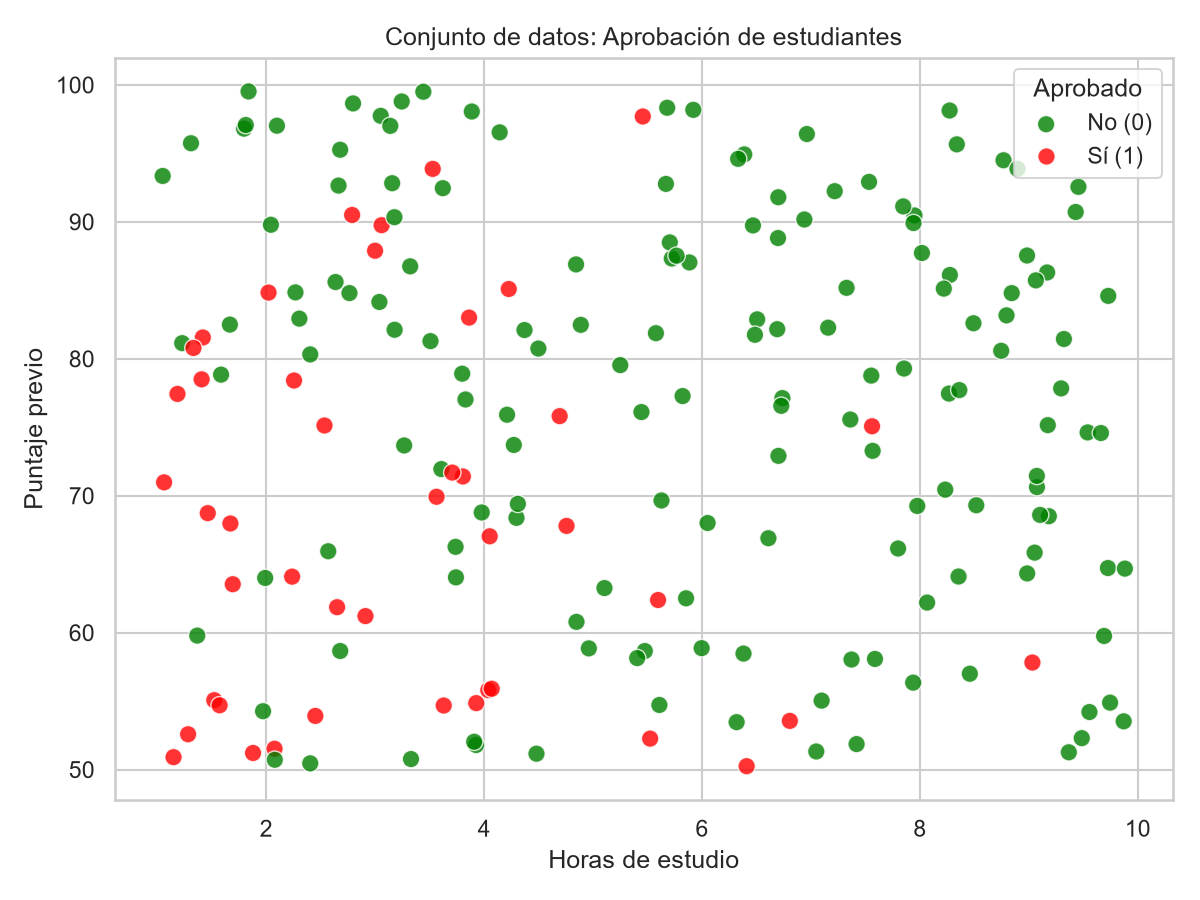
\includegraphics[width=0.5\linewidth]{Imagenes/Distribución_datos_sintét.png}
    \caption{Conjunto de datos sintético de 200 observaciones}
    \label{fig:placeholder1}
\end{figure}

\section{Métodos seleccionados}
Como se comentó anteriormente, se seleccionaron dos métodos iterativos de optimización sin restricciones, ambos aplicados directamente sobre la función de costo $J(\theta)$. Estos fueron seleccionados porque representan dos temas recurrentes en el curso: un método de primer orden y uno de segundo, su oposición interna permite ilustrar el compromiso central de la optimización numérica: costo por iteración frente a velocidad de convergencia. Parten del mismo punto inicial ($\theta = 0$) y del mismo criterio de parada por norma del gradiente, por lo que sus trayectorias de convergencia son comparables.

\subsection{Descenso del gradiente: primer método}
Es un método iterativo de optimización de primer orden que actualiza los parámetros en dirección del máximo decrecimiento de la función de costo, es decir, dirección opuesta al gradiente. Esta actualización sigue la regla:
\begin{equation}
\theta_{k+1} = \theta_k - \alpha \cdot \nabla J(\theta_k)
\end{equation}
Entonces, $\alpha$ es la tasa de aprendizaje, un número positivo que controla qué tan grande es el paso que damos en la dirección del gradiente; si $\alpha$ es muy pequeño, el método avanza muy lento y se necesitan muchas iteraciones, por el contrario, si es muy grande, se puede llegar a “saltar” el mínimo y el método puede oscilar o incluso divergir.

Este es un método de primer orden, pues solo usa información de la primera derivada (el gradiente), tiene convergencia lineal: el error se reduce en una fracción constante en cada iteración. Esto significa que, si se desea obtener una solución muy precisa, se necesitan bastantes iteraciones; además, la velocidad de convergencia depende de qué tan bien se elija $\alpha$ en relación con la curvatura de la función de costo (la cual es determinada por la segunda derivada o Hessiana), por lo que, en la práctica, el método es sensible a la escala de las variables y al valor de $\alpha$.

Se detiene cuando la norma del gradiente es menor que $\text{tol} = 1 \times 10^{-6}$, o al alcanzar la iteración 2000, con una $\alpha = 0.01$, un valor típico en la literatura para este tipo de problemas, aunque resultó insuficiente para lograr convergencia estable dado el desbalance de escalas entre variables.

El algoritmo implementado fue el siguiente:
\begin{enumerate}
    \item Construir la matriz de diseño $X$ añadiendo una columna de unos para el intercepto.
    \item Inicializar $\theta = 0$.
    \item Para cada iteración: calcular $\hat{y} = \sigma(X\theta)$, el gradiente $\nabla J(\theta)$, y actualizar $\theta$, registrando la pérdida en el historial.
    \item Detener el ciclo si $\|\nabla J(\theta)\| < \text{tol}$; en caso contrario, continuar hasta la máxima iteración permitida.
\end{enumerate}

\subsection{Método de Newton-Raphson}
Es un método iterativo de optimización de segundo orden que usa tanto el gradiente como la matriz Hessiana de la función de costo para construir una aproximación cuadrática local de $J(\theta)$ en cada iteración y salta directamente al mínimo de esa aproximación. Sigue la regla:
\begin{equation}
\theta_{k+1} = \theta_k - H(\theta_k)^{-1} \cdot \nabla J(\theta_k)
\end{equation}
Aquí, en vez de usar una tasa de aprendizaje fija, se calcula el tamaño de paso óptimo en cada iteración usando la curvatura de la función (la matriz Hessiana). En la práctica, en vez de invertir directamente la Hessiana se resuelve el sistema lineal:
\begin{equation}
H(\theta_k)\Delta\theta = \nabla J(\theta_k)
\end{equation}
para encontrar el paso $\Delta\theta$.

Su convergencia es cuadrática cerca del óptimo, pues el número de cifras decimales correctas se duplica aproximadamente en cada iteración. En problemas que tienen un comportamiento bueno, este método converge en pocas iteraciones (solo 7 en este caso); sin embargo, la desventaja es que cada iteración es más costosa computacionalmente, porque se debe construir y resolver un sistema lineal con la Hessiana.

La función debe ser dos veces diferenciable, con Hessiana definida, esta Hessiana debe ser invertible en cada iteración; en este caso, para evitar un mal comportamiento cuando las probabilidades predichas sean cercanas a 0 o 1, se añadió una regularización de Tikhonov ($H + \varepsilon I$, con $\varepsilon = 1 \times 10^{-6}$) antes de resolver el sistema. Y, por último, el punto inicial debe estar cerca del óptimo para así garantizar la convergencia cuadrática; en problemas convexos suele bastar partir desde 0.

El algoritmo implementado fue el siguiente:
\begin{enumerate}
    \item Construir la matriz de diseño $X$ añadiendo una columna de unos para el intercepto.
    \item Inicializar $\theta = 0$.
    \item Para cada iteración: calcular $\hat{y} = \sigma(X\theta)$, el gradiente $g$, la matriz $W$ y la Hessiana $H$, y actualizar $\theta$.
    \item Detener el ciclo si $\|g\| < \text{tol}$ (la misma que en el método anterior); en caso contrario, continuar hasta la máxima iteración permitida (50).
\end{enumerate}
Se escogió este método como contraparte de segundo orden pues, en un problema como este (baja dimensionalidad, tres parámetros), el costo de resolver un sistema $3 \times 3$ en cada iteración es insignificante frente a la ganancia en la velocidad de convergencia; especialmente al contrastarlo con el descenso del gradiente, cuya ventaja existe en problemas de alta dimensión donde construir la Hessiana es inviable, mientras que acá simplemente no converge.

\section{Implementación Computacional}

La arquitectura computacional del proyecto fue diseñada siguiendo principios de modularidad, reusabilidad y código limpio dentro del ecosistema de \texttt{Python 3}. El propósito principal de la librería \texttt{PyStatistics} es proveer una implementación transparente e independiente de los algoritmos de optimización para regresión logística, permitiendo un control preciso sobre las métricas internas de entrenamiento, la tolerancia numérica y el análisis de convergencia.

\subsection{Estructura del Proyecto y Módulos}
El código fuente se organizó bajo una estructura de paquete en el directorio \texttt{src/}, separando las responsabilidades de optimización, modelado y evaluación:

\begin{itemize}
    \item \texttt{src/optimizers/optimizer.py}: Define la interfaz y clase base abstracta \texttt{Optimizer}, la cual estandariza el contrato para los métodos de optimización (definiendo métodos como \texttt{fit} y \texttt{get\_history}).
    
    \item \texttt{src/optimizers/gradient\_descent.py}: Contiene la clase \texttt{GradientDescent}, encargada de ejecutar la optimización de primer orden mediante el cálculo vectorial del gradiente sobre la función de costo \textit{Log-Loss}.
    
    \item \texttt{src/optimizers/newton\_raphson.py}: Implementa la clase \texttt{NewtonRaphson}, la cual ejecuta la optimización de segundo orden incorporando el cálculo e inversión numérica de la matriz Hessiana para lograr una convergencia cuadrática.
    
    \item \texttt{src/models/logistic\_regression.py}: Modulo principal que define la clase \texttt{LogisticRegression}. Administra la transformación sigmoide, la adición del término de sesgo (\textit{bias/intercept}), la coordinación con el optimizador seleccionado y las funciones de predicción probabilística (\texttt{predict\_proba}) y binaria (\texttt{predict}).
\end{itemize}

\subsection{Entorno Computacional y Bibliotecas}
Para el desarrollo y soporte operativo de la solución se emplearon las siguientes bibliotecas especializadas:
\begin{itemize}
    \item \textbf{NumPy:} Empleada para el procesamiento matricial y operaciones algebraicas vectorizadas (productos punto, transposiciones e inversión de matrices), asegurando la eficiencia en la ejecución.
    \item \textbf{Pandas:} Utilizada en el estructurado y consolidado tabular de las métricas de desempeño y resultados comparativos.
    \item \textbf{Matplotlib y Seaborn:} Empleadas para la generación de gráficos técnicos, incluyendo la superficie de la función sigmoide, las fronteras de decisión y las matrices de confusión.
    \item \textbf{Scikit-Learn:} Utilizada exclusivamente como \textit{baseline} o modelo de referencia para la validación numérica de la implementación propia, empleando la clase \texttt{LogisticRegression} con el parámetro de regularización desactivado (\texttt{C=np.inf}) y el optimizador \texttt{solver='lbfgs'}.
\end{itemize}

\subsection{Decisiones de Implementación y Estabilidad Numérica}
Durante el desarrollo se tomaron decisiones clave para garantizar la estabilidad aritmética de los métodos:
\begin{enumerate}
    \item \textbf{Prevención de desbordamiento en la sigmoide:} Para evitar errores de tipo \textit{overflow} o \textit{underflow} al calcular $e^{-z}$ con valores extremos de $z$, se implementó un truncamiento numérico (\textit{clipping}) sobre el rango $[-50, 50]$.
    \item \textbf{Estabilidad en la \textit{Log-Loss}:} En el cálculo del logaritmo de las probabilidades ($\log(p)$ y $\log(1-p)$), se añadió una constante infinitesimal $\epsilon = 10^{-15}$ para evitar indefiniciones matemáticas ($\log(0)$).
    \item \textbf{Inversión de la Matriz Hessiana:} En la clase \texttt{NewtonRaphson}, el cálculo del paso $\mathbf{H}^{-1} \nabla J(\boldsymbol{\theta})$ se resolvió mediante el solucionador de sistemas lineales de NumPy (\texttt{np.linalg.solve}) en lugar de la inversión explícita directa, mejorando la precisión y la velocidad computacional.
\end{enumerate}

\subsection{Procedimiento de Verificación y Validación}
La validez del código se confirmó mediante un protocolo de dos etapas:
\begin{itemize}
    \item \textbf{Pruebas de consistencia interna:} Se verificó que la función de costo disminuyera monótonamente en cada iteración del historial (\texttt{history}) y que las probabilidades predichas se mantuvieran estrictamente acotadas en el intervalo $[0, 1]$.
    \item \textbf{Validación cruzada contra Scikit-Learn:} Se contrastaron los vectores de coeficientes ($\boldsymbol{w}$), el intercepto ($b$) y la función de pérdida final obtenidos por \texttt{PyStatistics (Newton-Raphson)} frente a la solución de \texttt{Scikit-Learn (L-BFGS)}, verificando una coincidencia numérica hasta el tercer decimal.
\end{itemize}

\section{Diseño de pruebas y experimentos}
El experimento consistió en entrenar el mismo modelo de regresión logística sobre el mismo conjunto de 200 observaciones, utilizando tres configuraciones de optimización: descenso del gradiente, con $\alpha = 0,01$ y un máximo de iteración de 2000, con una tolerancia de $1 \times 10^{-6}$. Newton-Raphson, con un máximo de iteraciones de 50 y misma tolerancia. Finalmente, Scikit-learn (L-BFGS), como solución de referencia de alta confiabilidad del proyecto.

Para ambas configuraciones se midieron las siguientes métricas sobre el conjunto completo de datos. Cabe aclarar que no se realizó una partición de entrenamiento o prueba, pues el objetivo es comparar la optimización numérica y no evaluar la capacidad de generalización del modelo, como fue definido como fuera del alcance en la sección 2.3:

- Número de iteraciones ejecutadas hasta la convergencia o hasta agotar el máximo permitido.

- Tiempo de cómputo total del ajuste.

- Exactitud, precisión, exhaustividad y F1-score de la clasificación resultante.

- Log-pérdida (entropía cruzada binaria) sobre las probabilidades predichas.

- Valor final del intercepto y los coeficientes, contrastados con el valor real ($b=-8$, $w_1 = 0,8$, $w_2 = 0,08$).

Adicionalmente, se registró el historial completo de la función de pérdida en cada iteración de ambos métodos, esto permite construir las curvas de convergencia y evaluar visualmente la estabilidad de cada trayectoria (sección 7.3.)

\section{Resultados}

Después de evaluar ambos modelos, se obtuvieron los siguientes resultados organizados en tablas:

\subsection{Tabla comparativa de métricas}
\begin{table}[H]
\centering
\begin{tabular}{|l|c|c|c|c|c|c|c|}
\hline
\textbf{Método} & \textbf{Iteraciones} & \textbf{Tiempo (s)} & \textbf{Accuracy} & \textbf{Precisión} & \textbf{Recall} & \textbf{F1-score} & \textbf{Log-Loss} \\
\hline
Descenso del gradiente & 2000 & 0,03867 & 0,78 & 0,780 & 1,0000 & 0,8764 & 1,1489 \\
Newton-Raphson & 7 & 0,00067 & 0,81 & 0,843 & 0,9295 & 0,8841 & 0,3925 \\
Scikit-learn & 26 & 0,01479 & 0,81 & 0,843 & 0,9295 & 0,8841 & 0,3925 \\
\hline
\end{tabular}
\caption{Métricas de desempeño de los métodos sobre el conjunto de 200 observaciones.}
\end{table}
\subsection{Parámetros estimados}
\begin{table}[H]
\centering
\begin{tabular}{|l|c|c|c|}
\hline
\textbf{Método} & \textbf{Intercepto ($b$)} & \textbf{$w_1$ (horas de estudio)} & \textbf{$w_2$ (puntaje previo)} \\
\hline
Valor real (tomado de la generación) & -8 & 0,8000 & 0,0800 \\
Descenso del gradiente & -0,5260 & 1,3123 & 0,0202 \\
Newton-Raphson & -4,8466 & 0,5220 & 0,0516 \\
Scikit-learn & -4,8464 & 0,5220 & 0,0516 \\
\hline
\end{tabular}
\caption{Comparación de los parámetros estimados por cada método frente al valor real usado para generar los datos.}
\end{table}
Newton-Raphson y scikit-learn coinciden hasta la tercera cifra decimal en los tres parámetros, ambos aproximándose razonablemente al valor real que fue generado, teniendo en cuenta que solo se hicieron 200 observaciones y existe ruido de muestreo. Por otro lado, el descenso del gradiente se aleja de manera considerable de ambos valores; esto indica que no alcanzó la convergencia.
\subsection{Explicación de la diferencia de iteraciones: Newton-Raphson vs. Scikit-Learn}
Se observa una diferencia representativa entre las 7 iteraciones empleadas por nuestra implementación de Newton-Raphson y las 26 iteraciones requeridas por Scikit-Learn (\texttt{solver='lbfgs'}). Esta disparidad no implica un menor desempeño por parte de Scikit-Learn, sino una diferencia conceptual en sus algoritmos de optimización:

\begin{itemize}
    \item \textbf{Newton-Raphson Puro (Segundo Orden Exacto):} Construye e invierte la matriz Hessiana exacta ($\mathbf{H} \in \mathbb{R}^{3 \times 3}$) en cada iteración . Al disponer de la curvatura exacta, logra una velocidad de convergencia cuadrática, requiriendo únicamente 7 iteraciones para alcanzar el mínimo de la función de costo.
    
    \item \textbf{Scikit-Learn (L-BFGS - Cuasi-Newton de Memoria Limitada):} No calcula ni invierte la matriz Hessiana real directamente. En su lugar, construye una aproximación iterativa de la curvatura utilizando únicamente la información de las diferencias de los gradientes de iteraciones previas. Como consecuencia de trabajar con una aproximación de la Hessiana, requiere un mayor número de pasos (26 iteraciones) para lograr la misma precisión final . Sin embargo, reduce drásticamente la carga computacional por iteración en problemas de alta dimensión.
\end{itemize}
\begin{table}[H]
\centering
\caption{Comparativa integral de desempeño, complejidad y vulnerabilidades entre los tres métodos de optimización.}
\label{tab:comparativa_3_metodos}
\resizebox{\textwidth}{!}{%
\begin{tabular}{|p{3.2cm}|p{4.2cm}|p{4.2cm}|p{4.5cm}|}
\hline
\textbf{Criterio / Método} & \textbf{Descenso del Gradiente (PyStatistics)} & \textbf{Newton-Raphson (PyStatistics)} & \textbf{Scikit-Learn (L-BFGS)} \\ \hline

\textbf{Orden de Optimización} & 
Primer orden (utiliza solo el gradiente $\nabla J(\boldsymbol{\theta})$) . & 
Segundo orden exacto (utiliza gradiente $\nabla J(\boldsymbol{\theta})$ y Hessiana $\mathbf{H}$) . & 
Cuasi-Newton (aproxima la Hessiana de forma iterativa) . \\ \hline

\textbf{Iteraciones Ejecutadas} & 
2000 (agota el máximo permitido sin converger) . & 
7 (convergencia cuadrática) . & 
26 (convergencia superlineal) . \\ \hline

\textbf{Tiempo de Cómputo (s)} & 
0,03867 s . & 
0,00067 s (el más rápido para este conjunto) . & 
0,01479 s . \\ \hline

\textbf{Log-Loss Final / Accuracy} & 
Log-Loss: 1,1489 \newline Accuracy: 0,78 . & 
Log-Loss: 0,3925 \newline Accuracy: 0,81 . & 
Log-Loss: 0,3925 \newline Accuracy: 0,81 . \\ \hline

\textbf{Costo por Iteración} & 
$\mathcal{O}(m \cdot p)$ \newline Muy bajo. Operaciones vectoriales simples . & 
$\mathcal{O}(m \cdot p^2 + p^3)$ \newline Extremadamente alto por la inversión/resolución de $\mathbf{H}$. & 
$\mathcal{O}(m \cdot p + m \cdot k)$ \newline Moderado-Bajo. Guarda solo los últimos $k$ gradientes. \\ \hline

\textbf{Peligros y Sensibilidades} & 
- Alta sensibilidad a la tasa de aprendizaje ($\alpha$) . \newline
- Falla grave ante variables sin escalamiento/normalización . & 
- Inviable en alta dimensión ($p > 10.000$ variables) por almacenamiento y cómputo de $\mathbf{H}$. & 
- Ligeramente dependiente del parámetro de memoria $k$ guardado. \\ \hline

\textbf{Casos de Falla y Vulnerabilidad} & 
- Oscilación e inestabilidad (zigzagueo constante) . \newline
- Clasificación sesgada (predijo el 100\% a favor de una sola clase) . & 
- Mal funcionamiento si la Hessiana es singular ($\det(\mathbf{H}) \approx 0$) o mal condicionada . & 
- Pérdida de precisión si la función de pérdida no es suave o presenta bastante ruido. \\ \hline
\end{tabular}%
}
\end{table}
\subsection{Curvas de convergencia}

\begin{figure}[H]
    \centering
    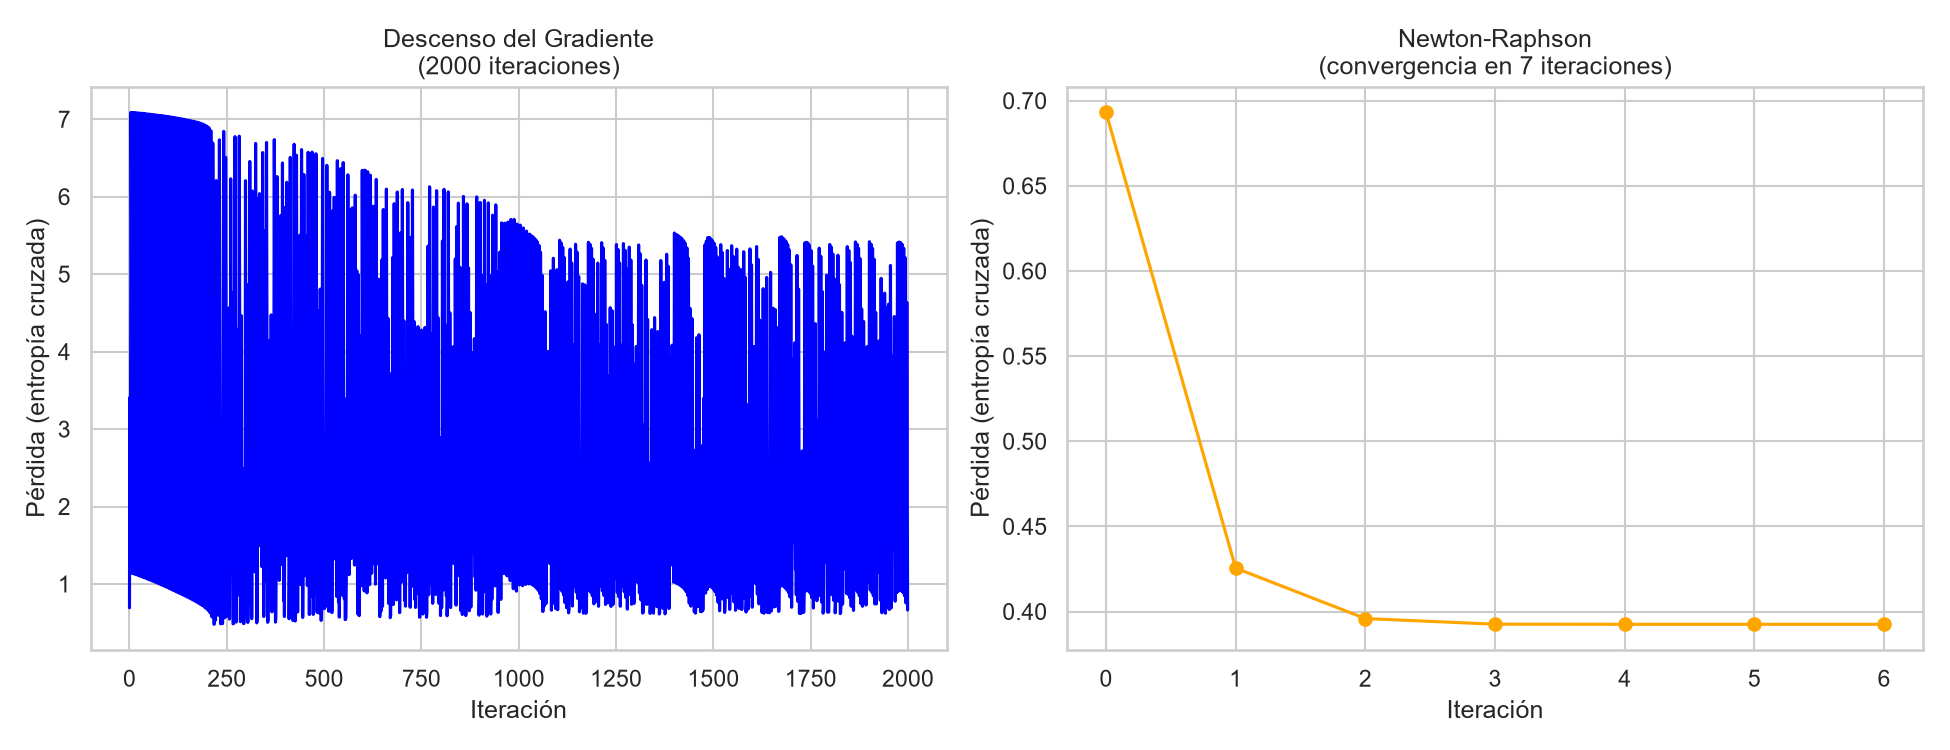
\includegraphics[width=0.8\linewidth]{Imagenes/CURVAS_convergencia.png}
    \caption{Evolución de la función de pérdida en cada iteración para el descenso del gradiente (izquierda) y Newton-Raphson (derecha). Nótese la diferencia de escala en el eje horizontal.}
    \label{fig:placeholder2}
\end{figure}

Sin entrar en detalles, se observa una gran diferencia en el comportamiento de ambos métodos. Esto es aún más evidente en la siguiente gráfica, donde se juntan ambas convergencias en la misma escala:

\begin{figure}[H]
    \centering
    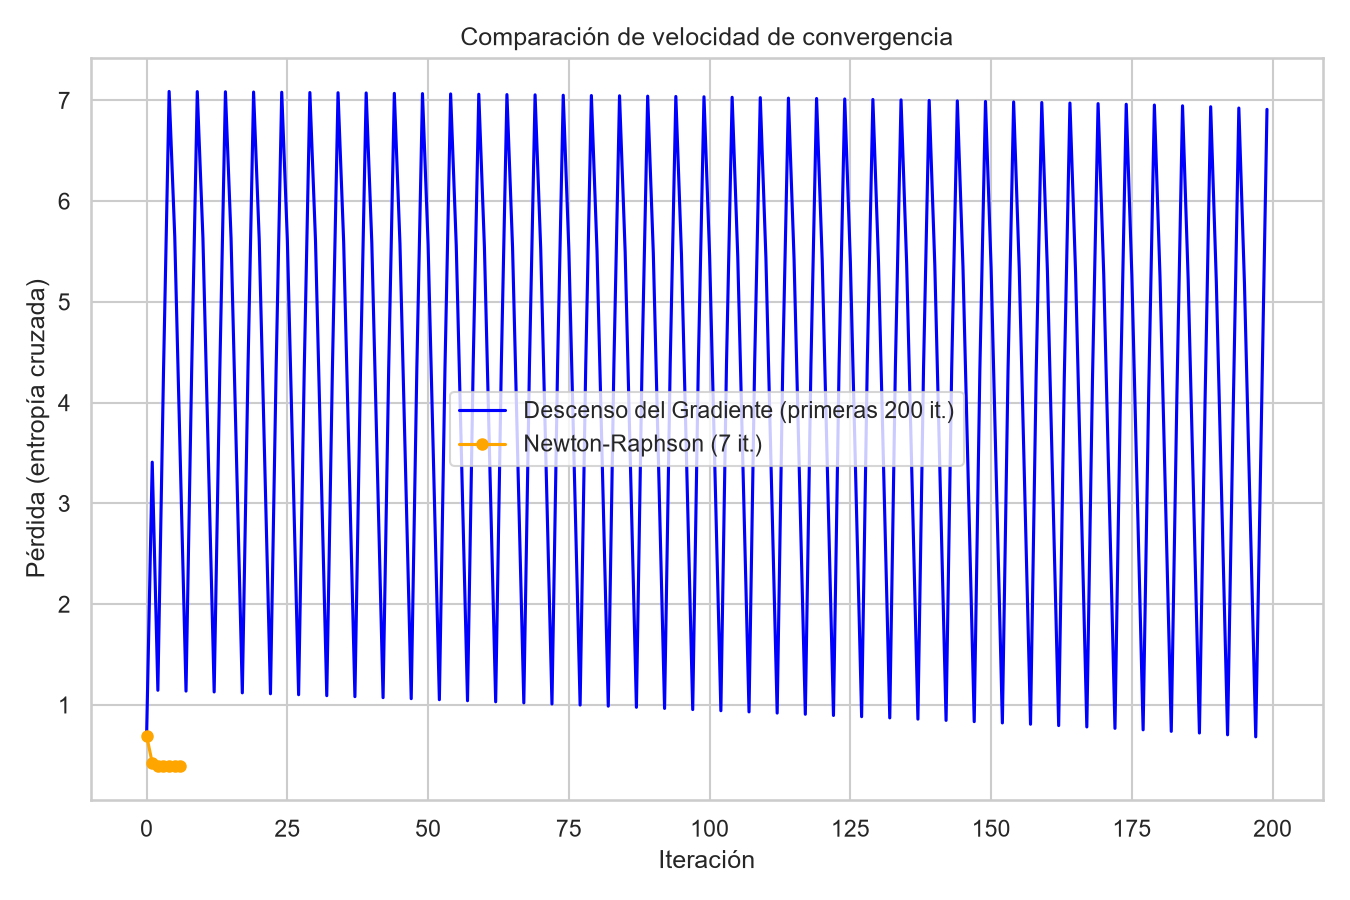
\includegraphics[width=0.5\linewidth]{Imagenes/_convergencia_zoom.png}
    \caption{Comparación directa de la velocidad de convergencia en las mismas unidades de pérdida.}
    \label{fig:placeholder3}
\end{figure}
\subsection{Fronteras de decisión}

\begin{figure}[H]
    \centering
    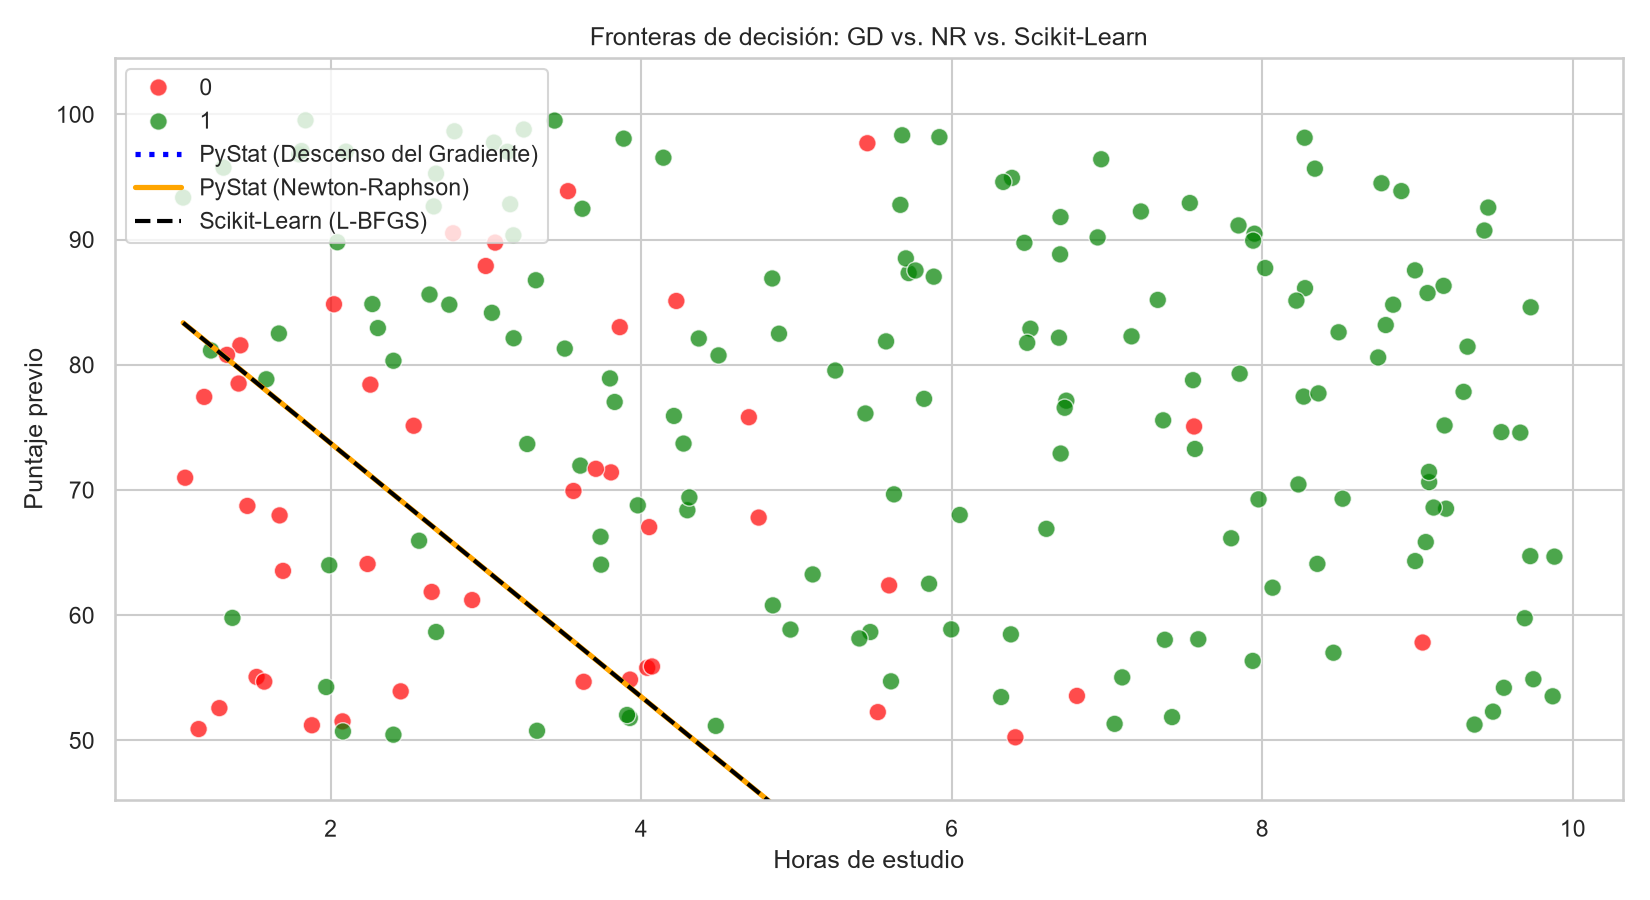
\includegraphics[width=0.7\linewidth]{Imagenes/fig3_fronteras.png}
    \caption{Fronteras de decisión obtenidas por los tres métodos, superpuestas sobre el conjunto de datos. Nótese que, en el rango tomado, la encontrada por el descenso del gradiente ni siquiera es visible.}
    \label{fig:placeholder4}
\end{figure}

La frontera obtenida por Newton-Raphson es visualmente indistinguible de la de Scikit-learn, mientras que, la obtenida por el descenso del gradiente ni siquiera es visible en la figura, pues sus valores son tan alejados que cae en valores de puntaje previos entre $-3$ y $-50$ para el rango de horas de estudio graficado, lo que no solo es bastante alejado del eje visible, sino que no tiene sentido físico; esto, como se verá posteriormente, termina clasificando a todos los estudiantes como aprobados sin distinguir realmente cuáles o hicieron o no (Figura 4.)

\subsection{Matrices de confusión}

Una matriz de confusión es una tabla que muestra los aciertos y los errores de los resultados de un algoritmo clasificador. En este caso, las obtenidos para el proyecto fueron:

\begin{figure}[H]
    \centering
    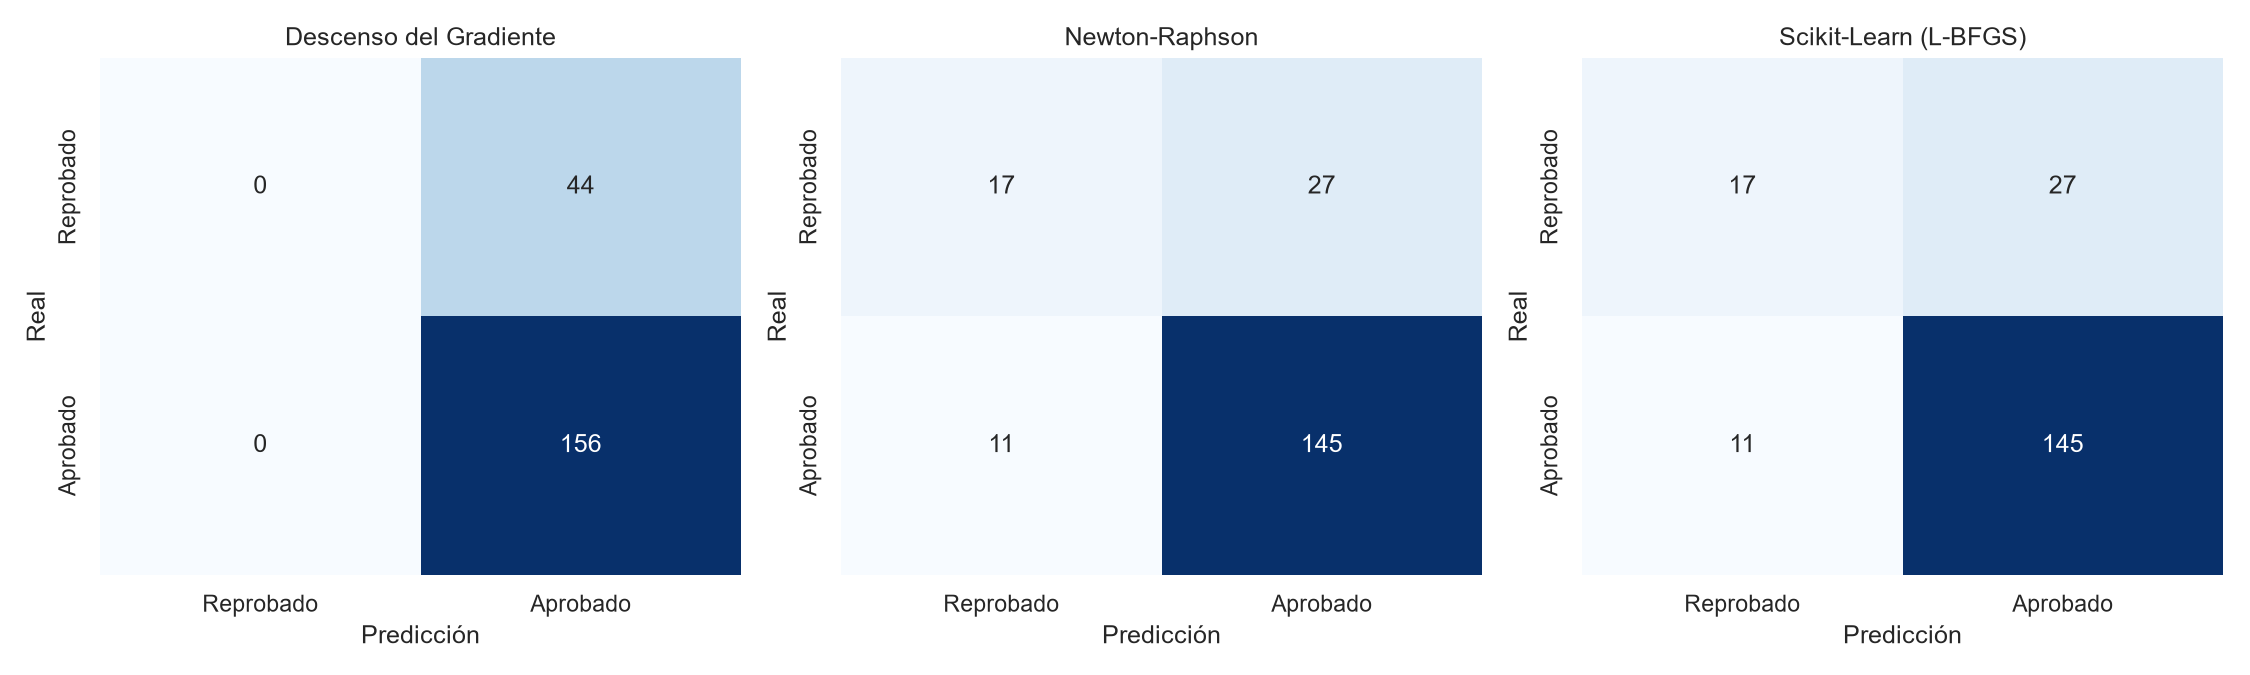
\includegraphics[width=0.8\linewidth]{Imagenes/fig4_matrices_confusion.png}
    \caption{Matrices de confusión de los tres métodos sobre el conjunto de 200 observaciones.}
    \label{fig:placeholder5}
\end{figure}

La matriz de confusión del descenso del gradiente muestra que el método clasifica correctamente a todos los estudiantes en 1 (recall=1,0), pero esto lo hace sin importar clasificar erróneamente a una fracción importante de los negativos (desaprobados) reales (con una precisión de 0,78), esto es consistente con el desplazamiento de la frontera al no haber convergido. Por otro lado, Newton y Scikit-learn producen matrices prácticamente idénticas y un mejor balance entre falsos negativos y falsos positivos.

\section{Análisis comparativo entre ambos métodos}

\subsection{Precisión y error}

Newton-Raphson alcanza una log-loss de 0,3925, curiosamente idéntica hasta la cuarta cifra decimal a la de scikit-learn, y una exactitud de 0,81. El descenso del gradiente, después de agotar el máximo de iteraciones, alcanza un log-loss muy superior (por encima de 5 en sus últimas iteraciones) y una exactitud ligeramente menor (0,78). Esto evidencia que, con los parámetros usados, no logró aproximarse óptimamente de manera remotamente similar a como lo hizo un método de segundo orden.

\subsection{Rapidez y costo computacional}

En cuanto al número de iteraciones, Newton-Raphson requirió solo de 7, frente a las 2000 agotadas por el descenso del gradiente. Sin embargo, se debe tener en cuenta que el costo por iteración de Newton es mucho mayor, pues cada paso implica construir una Hessiana 3x3 y resolver un sistema lineal, mientras que cada paso en el gradiente solo requiere un producto matriz-vector. En este problema específico, este costo adicional es prácticamente insignificante frente a la velocidad de convergencia del método, resultando en un tiempo menor. Sin embargo, es un factor a tener en cuenta en problemas de alta dimensionalidad, donde construir y resolver un sistema con el Hessiano puede ser engorroso o complejo, en estas situaciones, el bajo costo del descenso del gradiente lo hace la opción óptima para la resolución.

\subsection{Convergencia y estabilidad}

La figura 2 muestra el contraste entre ambos métodos, la curva de Newton-Raphson muestra una caída rápida y monótona de la pérdida, que se estabiliza cerca de 0,4 después de 7 iteraciones. Por otro lado, la curva del descenso del gradiente no muestra una tendencia sostenida: inicialmente desciende, pero luego oscila entre valores muy altos y muy bajos. Este comportamiento no parece atenuarse a medida que se acerca a las 2000 iteraciones, lo que indica no convergencia; además, evidencia que el tamaño de paso seleccionado es demasiado grande para la dirección de mayor escala (puntaje previo) y demasiado pequeño para la de menor escala (horas de estudio). Este comportamiento extraño del descenso del gradiente es común cuando las variables explicativas tienen escalas muy distintas y no son normalizadas antes.

\subsection{Sensibilidad a parámetros e hiperparámetros}

En este problema, NR es relativamente insensible al punto de partida y no requiere ajustar ningún hiperparámetro de tamaño de paso; a diferencia del DDG, el cual es bastante sensible a la elección de $\alpha$: si se escogiese un valor más pequeño, eliminaría la oscilación, pero requeriría más iteraciones, mientras que un valor más grande provocaría divergencia. Ya sensible de por sí, es agravada por la diferencia de escala entre las variables (de aproximadamente un factor de 10 entre ambas), que hace que no exista un único $\alpha$ adecuado para ambas direcciones sin antes normalizar los datos.

\section{Discusión}

Los resultados son consistentes con la teoría de optimización numérica, que establece que, para funciones convexas y de baja dimensionalidad, los métodos de segundo orden como Newton-Raphson aprovechan la información de curvatura para converger en menos iteraciones, esto a costa de una iteración más robusta y engorrosa que, en este caso, resulta insignificante cuando el número de parámetros es pequeño. El resultado más evidente es el fallo del descenso del gradiente; sin embargo, se destaca que este no falló por un error de implementación, sino por una limitación importante del método: su sensibilidad al escalamiento relativo de las variables. Esto sugiere que, si se repitiese el experimento con las variables normalizadas, este podría lograr converger de forma estable con la misma tasa de aprendizaje, lo que es fuertemente apoyado por el equipo de trabajo como trabajo futuro.

Además, una limitación adicional es que el desempeño de cada método dependió directamente del conjunto de datos usado para entrenar el modelo, sin una partición de validación independiente o de prueba; lo cual es adecuado para el objetivo del proyecto, que solo se enfoca en comparar las optimizaciones y no en la capacidad de generalización del modelo; sin embargo, esto implica que la exactitud de 0,81 que se reporta no puede interpretarse como una estimación de lo que pasaría si el modelo se usase con estudiantes reales o datos distintos a los usados. Otra limitación es que el problema solo tiene tres parámetros, lo que significa una ventaja casi garantizada para NR, como se mencionó antes, si los parámetros aumentasen, la rigurosidad de Newton sería muchísimo más determinante en qué método escoger.

\section{Conclusiones y recomendaciones}

En respuesta al objetivo general planteado, se concluye que, para el caso estudiado (tres parámetros, 200 observaciones, variables sin normalizar), el método de Newton-Raphson es claramente superior al Descenso del gradiente: converge en 7 iteraciones frente a las 2000 agotadas por el segundo, alcanza una log-loss y una exactitud prácticamente idénticas a las de Scikit-learn, y su costo adicional es sopesado por esta misma velocidad de convergencia, dado la baja dimensionalidad del problema; es el método más robusto, preciso y rápido, sin desventajas prácticas relevantes. Por otro lado, el Descenso del Gradiente, usando un $\alpha = 0.01$, no logró converger de forma estable en el máximo de iteraciones permitido. Esto evidencia una limitación bastante importante de los métodos de primer orden con paso fijo: su desempeño depende mucho del preprocesamiento de los datos y del correcto ajuste de la tasa de aprendizaje, responsabilidad del usuario que implementa el algoritmo y no del algoritmo en sí. Implica que, si se desea que este método sea viable en problemas como este, se necesitan modificaciones adicionales, por ejemplo, normalizar las variables o lograr una tasa de aprendizaje adaptativa. Como recomendaciones para un trabajo futuro se propone: 
- Repetir el experimento normalizando las variables explicativas para verificar si el Descenso del gradiente logra converger de forma estable con la misma tasa de aprendizaje. 
- Explorar una tasa de aprendizaje adaptativa o variantes del método (momentum, Adam) que sean más robustas a diferencias de escala entre variables. 
- Extender la comparación a un problema donde exista una mayor dimensionalidad, donde la ventaja previa de NR se reduzca o incluso revierta, debido al costo de construir y resolver el Hessiano. 
- Para un caso real, incorporar un primer entrenamiento para evaluar la capacidad de generalización del modelo, para así poder complementar el análisis de optimización numérica.

\section{Contribución de los integrantes}

Sofía González: Redacción del documento escrito, planteamiento matemático, generación y análisis de las figuras. 

Nicolás Godoy: Implementación y creación del algoritmo en su totalidad, implementación de los optimizadores GradientDescent y NewtonRaphson, redacción de la sección 5 (implementación computacional). 

Ambos integrantes participaron en la revisión final del informe y en la preparación de la presentación tipo pitch para la sustentación del proyecto.

\vspace{0.5cm}

\noindent El código fuente completo (paquete \texttt{src/}, con los módulos \texttt{optimizar.py}, \texttt{gradient\_descent.py}, \texttt{newton\_raphson.py} y \texttt{logistic\_regression.py}), junto con las instrucciones referentes al desarrollo y validación de los algoritmos, se encuentran disponibles en el repositorio oficial de GitHub y en la carpeta de soporte adjunta a esta entrega.

\vspace{0.3cm}
\noindent \textbf{Instrucciones de ejecución:} 

 Para reproducir completamente los resultados y experimentos presentados en este informe, siga los pasos a continuación desde la terminal o consola de comandos:

\begin{enumerate}
    \item \textbf{Clonar el repositorio oficial desde GitHub:}
    \begin{verbatim}
git clone https://github.com/ngodoya/Metodos-Numericos-Proyecto.git
cd Metodos-Numericos-Proyecto
    \end{verbatim}

    \item \textbf{Crear y activar un entorno virtual (recomendado):}
    \begin{verbatim}
python -m venv venv
# En Linux/macOS:
source venv/bin/activate
# En Windows (PowerShell):
.\venv\Scripts\Activate.ps1
    \end{verbatim}

    \item \textbf{Instalar las dependencias del proyecto:}
    \begin{verbatim}
pip install -r requirements.txt
    \end{verbatim}

    \item \textbf{Ejecutar el cuaderno interactivo de Jupyter:}
    \begin{verbatim}
jupyter notebook
    \end{verbatim}
    Abra el archivo \texttt{notebooks/benchmarking.ipynb} o el cuadernillo principal para ejecutar secuencialmente todas las celdas de pruebas y generar las gráficas de soporte.
\end{enumerate}


\bibliography{referencias}
%%------------------------------- contribution acknowledgements page ----------------------------------

\thispagestyle{declarationstyle}
\vspace*{12mm}




\end{document}